\let\textcircled=\pgftextcircled
\chapter{Introduction}
\label{chap:intro}

\initial{N}atural language processing is being increasingly used by different organisations to  improve the dialogue with the customers, efficiently analyse the opinion about a number of topics while using the existing social media tools, and offer additional services which would not have been possible without computational linguistics - such as speech recognition. In a way, Natural Language Processing allows the organisations using social media to have an additional sensor of the public opinion without asking people to give explicit feedback.

Natural Language Processing is becoming a tool that allows to systematise, organise and process huge amount of unstructured data which has been one of the biggest problems of the digital world. One of the applications of these techniques could be to create a seamless experience for the people living in a certain council area to communicate with the estate, provide feedback and receive answers to their questions. The main advantage of such a technique is the fact that such organisations can use already existing popular social media platforms such as Twitter and Facebook and can avoid setting up their own separate communication channel. 

%=======
\section{Falkirk Council and Grangemouth}
\label{sec:falkirk}

Grangemouth is a Scottish town and is a part of the Falkirk council area. Its population was estimated to be around 17000 people by the 2011 census \cite{grangemouthcensus}. The growth of the town has mostly been defined by its location: Grangemouth was a port and used to play an important part in trading and the transportation of the imported goods using the Forth and Clyde Canal. Nowadays, a lot of the town production is defined by the oil refinery, which is commonly called Grangemouth, too, and has changed its owners several times in the last decades.

\subsection{Environmental Issues in Grangemouth}
\label{subsec:environment}

\subsection{Grangemouth in Social Media}
\label{subsec:media}

\section{Project Objectives}
\label{sec:objectives}

\section{Extent of completeness}
\label{sec:completeness}

% %A figures matrix.
% \begin{figure}[t!]
% \centering
% \begin{minipage}{3.3cm}
%     \centering
%     \subtop[]{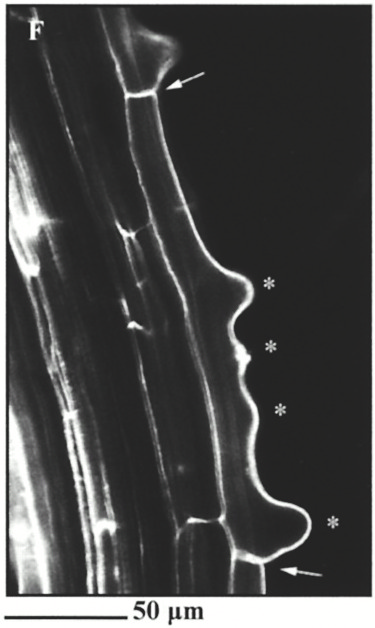
\includegraphics[height=0.28\textheight]{fig01/Nswellings}\label{sf:multiRH02a}}
% \end{minipage}
% \hspace{0.5cm}
% \begin{minipage}{3.3cm}
%     \centering
%     \subtop[]{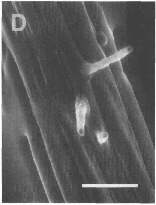
\includegraphics[height=0.27\textheight]{fig01/Mswellings}\label{sf:multiRH02b}}
% \end{minipage}
% \hspace{1.3cm}
% \begin{minipage}{10cm}
%     \centering
%     \subtop[]{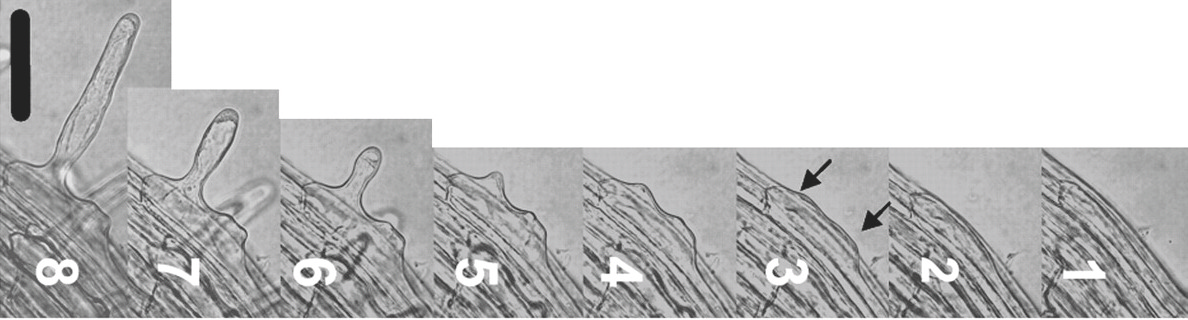
\includegraphics[height=0.145\textheight]{fig01/mutantrhd6}\label{sf:multiRH02d}}
% \end{minipage}
% \\ \vspace{0.1cm}
% \begin{minipage}{10cm}
%     \centering
%     \subtop[]{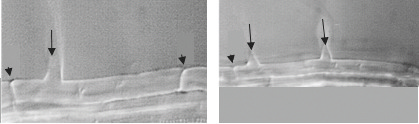
\includegraphics[height=0.16\textheight]{fig01/auxab}\label{sf:multiRH02e}}
% \end{minipage}
% \mycaption[Hair-forming mutant cells.]{(a) A mutant RH cell. (b)~Hair-forming cell with three RH initiation locations. (c) Large bump in mutant {\itshape rhd1}. (d) Mutant overexpressing gene {\itshape ROP2}}
% \label{fig:multiRH02}
% \end{figure}

% % A single figure
% \begin{figure}[t!]
% 	\centering
% 	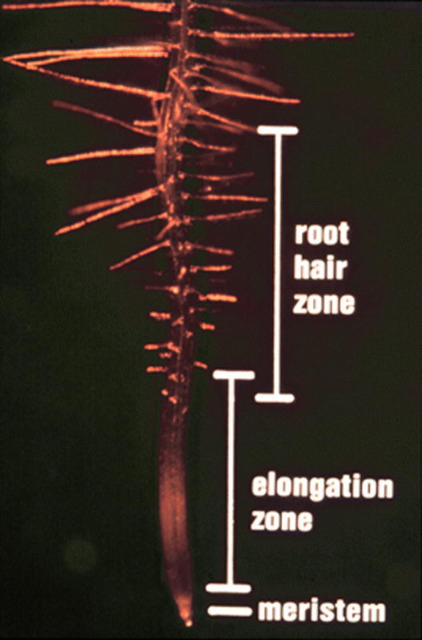
\includegraphics[height=0.35\textheight]{fig01/devepzones}
% 	\mycaption[Developmental zones of an Arabidopsis root.]{Developmental zones of an Arabidopsis root. Figure reproduced from \cite{griersonRH}.}
% 	\label{fig:RHP02}
% \end{figure}

%=========================================================